\begin{figure}[H]
    \centering
    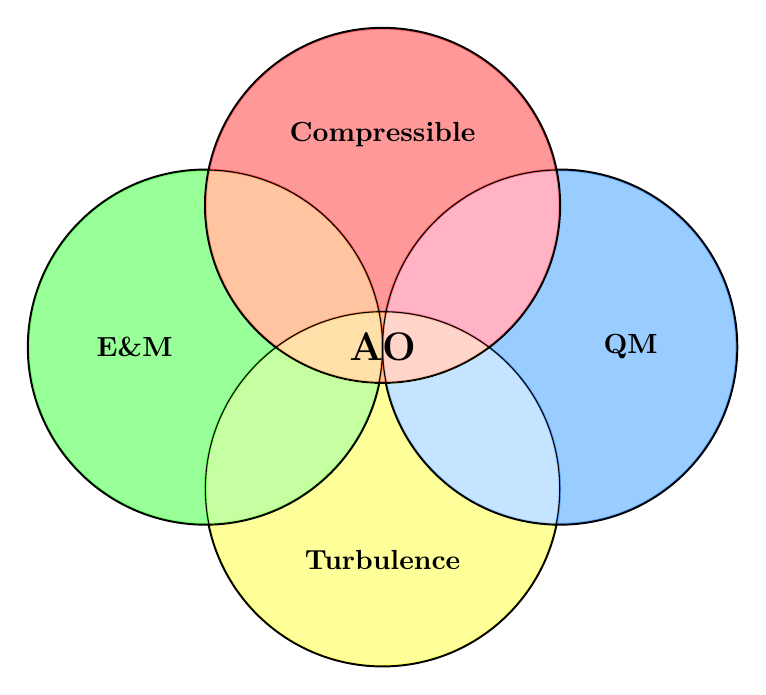
\begin{tikzpicture}[scale=0.9]
     % Define colors
        \definecolor{circleA}{RGB}{255, 153, 153} % Light Red
        \definecolor{circleB}{RGB}{153, 204, 255} % Light Blue
        \definecolor{circleC}{RGB}{153, 255, 153} % Light Green
        \definecolor{circleD}{RGB}{255, 255, 153} % Light Yellow

        % Draw four overlapping circles
        \begin{scope}[blend group = soft light]
            \filldraw[fill=circleA]  (0,1.5) circle (2.5cm); % E&M
            \filldraw[fill=circleB]  (2.5,-0.5) circle (2.5cm); % QM
            \filldraw[fill=circleC]  (-2.5,-0.5) circle (2.5cm); % Compressible
            \filldraw[fill=circleD]  (0,-2.5) circle (2.5cm); % Turbulence
        \end{scope}

        % Draw the circle outlines
        \draw (0,1.5) circle (2.5cm);
        \draw (2.5,-0.5) circle (2.5cm);
        \draw (-2.5,-0.5) circle (2.5cm);
        \draw (0,-2.5) circle (2.5cm);

        % Add text labels
        \node at (0,2.5) {\textbf{Compressible}};
        \node at (3.5,-0.5) {\textbf{QM}};
        \node at (-3.5,-0.5) {\textbf{E\&M}};
        \node at (0,-3.5) {\textbf{Turbulence}};
        
        % Central AO text in the overlapping region
        \node at (0,-0.5) {\Large \textbf{AO}};
    \end{tikzpicture}
    \caption{\gls{AO} Venn Diagram\label{fig:aoVennDiagram}}
\end{figure}
